

\chapter{Cryptanalysis}

\section{Security goals viewed by Cryptanalysis}
	\begin{itemize}
		\item In general, security of crypto primitives can be hard to define
		\item « Extreme definitions » don’t work, exemple:
		\begin{itemize}
			\item Secret key should be impossible to find\\
			$\Rightarrow$ Too weak
			\item A Block cipher should behave in all respects like a random permutation\\
			$\Rightarrow$ Impossible to achieve
		\end{itemize}
		\item Security proofs need formal definition. Cryptanalysts don’t!
		\item Basically, any « non generic » property might become a weakness
		\begin{itemize}
			\item Some generic properties might also be weaknesses showing bad parameters
		\end{itemize}
	\end{itemize}
	A first remark is that security notions are not intuitive in the field of cryptology. 
	Even the meaning of the word « attack » is relative and shifts with time or with respect to the point of view of the speaker. 
	In particular, the security notions involved in security proofs can be very different from the one we see in cryptanalysis. 
	For security proofs, a formal definition is required; for cryptanalysts, an attack scenario with a potential weakness that could be exploited is a better justification. 
	The choice of scenario has greatly evolved with time. 
	In the early days of historical crypto, ciphertext-only attacks were the reference.
	Nowadays, a wide range of interactive attacks are considered.\\
	For this reason, just asking for the secret-key to be impossible to recover by an attacker isn’t enough. 
	It might not prevent them from deciphering messages or from performing unauthorised modifications. 
	At the other extreme, some definitions can be too strong, simply because they are impossible to achieve. 
	We give an example in the next slide.\\
	The current consensus among secret-key cryptographers is that any explicit, non-generic, 
	property of a cryptographic primitive is a potential weakness (at least, as long as it can be made explicit with an efficient enough computation). 
	In some cases, generic weaknesses simply show that some desired primitive is just impossible to construct in a secure way.

\section{Block Ciphers}
	\begin{center}
		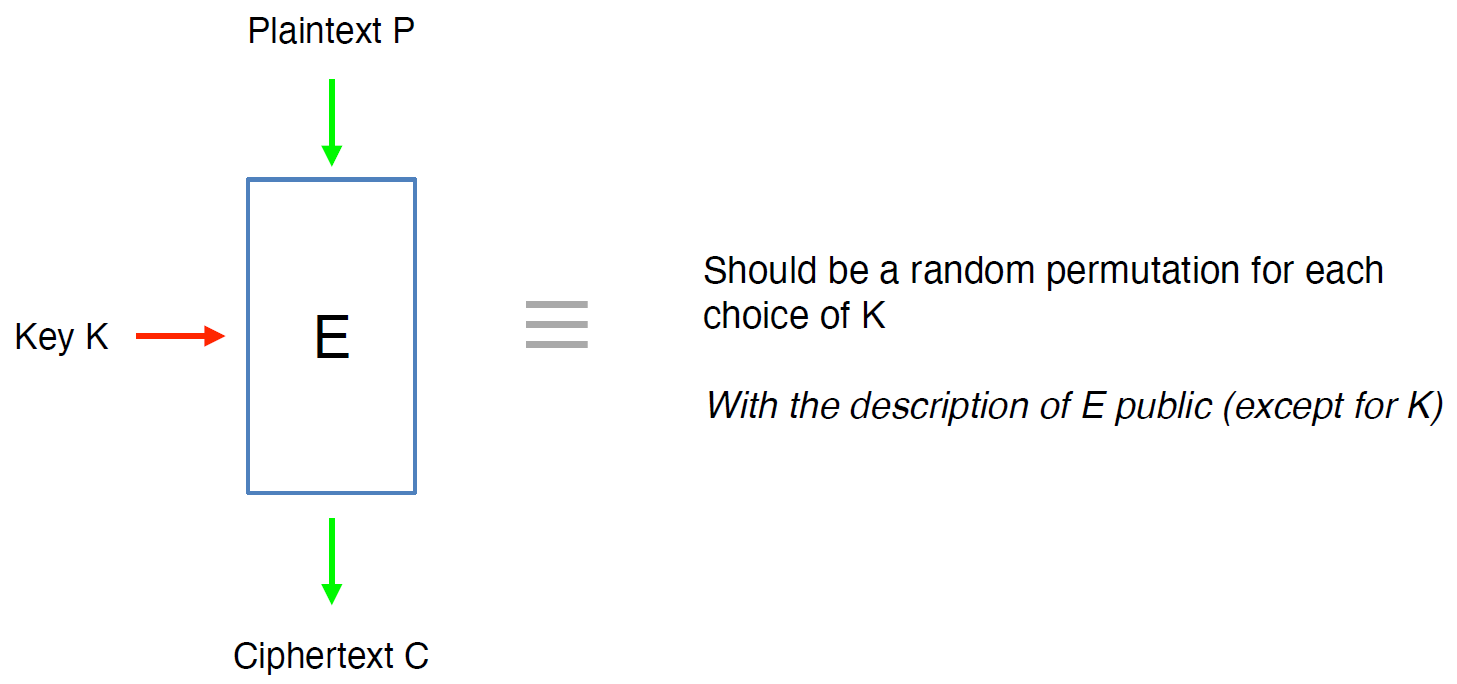
\includegraphics[width=140mm]{Graphics/Cryptanalysis/c1.png}
	\end{center}
	A first idea would be to request that a block cipher should behave like a random permutation in all respects for every choice of the key K. 
	Furthermore, following Kerckoffs’ principle, we still want this to be true when the description of the cipher itself is public and only the key remains secret.
	\begin{itemize}
		\item This informal definition is impossible to achieve
		\begin{itemize}
			\item Indeed, a random permutation doesn’t generally have a compact description
		\end{itemize}
		\item Generic attacks
		\begin{itemize}
			\item Exhaustive key search
			\item Plaintext block collisions are visible on Ciphertext block
		\end{itemize}
		\item[$\Rightarrow$] Key size and block size should be large enough. Today’s standard:
		\begin{itemize}
			\item At least 128 bits for key size, 192 or 256 are better when possible
			\item At least 128 bits for block size\\
			(64 bits still appears in legacy applications)
		\end{itemize}
	\end{itemize}
	Unfortunately, this definition cannot be achieved. 
	Indeed, by construction the block cipher has a compact description (in the form of its program), which is impossible for a truly random permutation.\\
	Instead, for security proofs, one turns to the notion of random permutation family which we will not revisit during this lecture.\\
	Since a block cipher is a permutation acting on plaintext-block values and chosen in a large but finite family by instantiating the key, some generic attacks arise. 
	First, since there are only finitely many keys, an attacker could (in principle) try all of them to recover the correct one. 
	Due to Shannon’s information theory, even a few blocks of data are enough to uniquely characterise the correct key. 
	To make this attack infeasible, cryptographers use extremely large sets of possible keys. 
	The current choice of key size is between 128 and 256 bits. 
	As a consequence, exhaustive search is infeasible even for attackers possessing tremendous computing powers and willing to use them for years or even decades.\\
	Another generic property is that encrypting the same block of plaintext twice yields the same ciphertext. 
	This can lead to devastating attacks. 
	As a consequence, block-ciphers always need to be used in a way that prevents such collisions between plaintext values from occurring. 
	This is taken into account when constructing « modes of operation », which are basically recipes for using block ciphers. 
	Furthermore, the block size should be large enough to prevent collisions from appearing when blocks are randomly chosen. 
	For this reason, modern block ciphers operate on 128 bits at a time.

\newpage
\section{DES}
	\subsection{DES: an outdated but interesting example}
		\begin{itemize}
			\item DES = Data Encryption Standard
			\item Block Cipher developed in the 70s at IBM
			\item NIST standard from 1976 to 2005
			\item DES is a Feistel cipher with a 56-bit key and 64-bit blocks
			\item Even in 1976, the key size was on the low side
		\end{itemize}
		During this lecture, we are going to use DES as an example to present some cryptanalytic results. 
		Despite being outdated, this algorithm has motivated a lot of research in cryptanalysis and led to several seminal breakthroughs. 
		In addition, since it was a NIST standard from 1976 to 2005, it is still often encountered in legacy applications. 
		This cipher has 56-bit keys and 64-bit blocks. 
		Note that even when it is was introduced, its key size was already considered too small by many people in academia.
	
	\subsection{How to have longer keys?}
		\begin{itemize}
			\item Modify the algorithm to change key size
			\begin{itemize}
				\item In the long run, it led to AES (Advanced Encryption Standard)
				\item In the early days, FEAL tried to improve on DES
			\end{itemize}
			\item Incorporate the algorithm in a bigger structure:
			\begin{itemize}
				\item Multiple DES (Introduced by Diffie-Hellman 77)
				\item DES-X (Rivest’84, unpublished)
			\end{itemize}
		\end{itemize}
		Because of DES small key size, the question of increasing the key size quickly arose. 
		One obvious avenue is to redesign a new cipher with bigger keys. 
		However, the crypto community soon discovered that this is harder than it seems and many attempts were broken which helped slowly building cryptanalytic expertise within academia.
		Eventually, NIST even became confident that this expertise was very strong and asked the community to design the successor of DES in the open AES competition.\\
		Another avenue is to assume that DES is well-designed, despite its small key, and to integrate it into a bigger construction to obtain larger keys.
	
	\subsection{Multiple DES - Diffie-Hellman 77}
		Another way to obtain a variable length key would be to use the currently proposed standard, but to encipher $m$ times with $m$ independent 56-bit keys.
		This would hopefully yield a 56$m$-bit key, but additional analysis is required.
		For example, enciphering twice with two monoalphabetic ciphers is equivalent to enciphering only once with a third monoalphabetic cipher.
		If cipher one carries $A$ to $F$ and cipher two carries $F$ to $C$, then the overall effect is to carry $A$ to $C$.
		This is because monoalphabetic ciphers form a semi-group under composition.
		It is highly doubtful that the proposed standard possesses this property.\\
		
		A first method, proposed by Diffie and Hellman in 1977 is simply to encrypt several times with independent keys. 
		They remarked that if DES was hiding a group-like structure, this approach would be doomed. 
		It took some time for the community to rule out this possibility.

\newpage
	\subsection{Double DES - Diffie-Hellman 77}
		After introducing multiple DES, they show that m=2 isn’t secure
		\begin{center}
			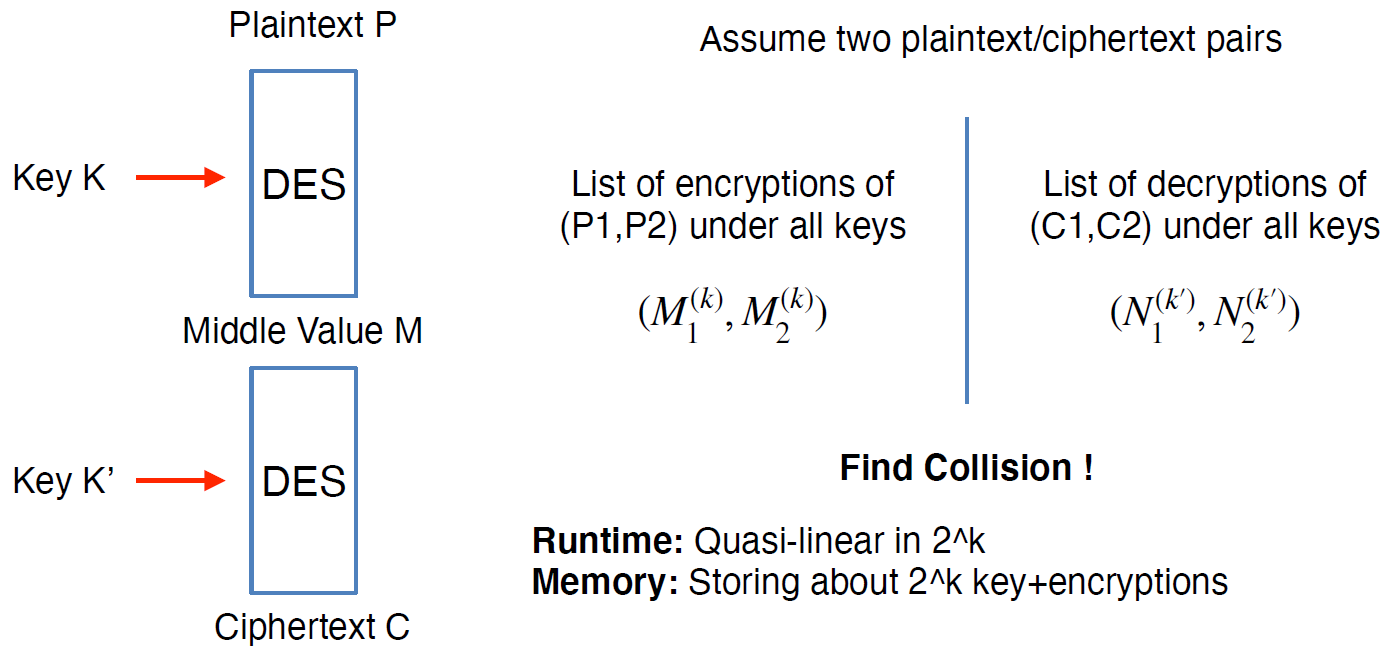
\includegraphics[width=140mm]{Graphics/Cryptanalysis/c2.png}
		\end{center}
		In the same paper, Diffie and Hellman show that encrypting twice isn’t good enough and doesn’t provide the security level that one should expect from 112-bit keys. 
		To see that, assume that we know the encryption of two plaintext blocks. 
		Indeed, one isn’t enough to characterise the key of double DES.
		Remark that if we encrypt the plaintext with the first half of the key and decrypt the ciphertext with the second half, we obtain the same middle values. 
		Moreover, for wrong keys, this event is really unlikely.\\
		
		As a consequence, we construct two lists, the first with all encryptions under all first half-keys and the second with all decryptions. 
		We expect very few collisions between these lists and every collision give a candidate key. 
		The right key is, of course, within this small set and it is easy to test it (for example by decrypting some extra text). 
		This works because collisions can be found efficiently.


\section{Finding Collisions in a list or between lists}
	\begin{itemize}
	    \item This is a major algorithmic tool in cryptanalysis
	    \item Can be done in quasi-linear time in the lists’ sizes\\
	    \item Basic idea for a single list:
	    \begin{itemize}
	        \item Sort the list of size $N$ (takes $O(N \cdot log(N))$ comparisons)
	        \item Read it in order. Collisions will be between consecutive elements!
	        \item Any ordering of the elements work (a natural ordering isn’t needed)\\
	    \end{itemize}
	    \item With two lists:
	    \begin{itemize}
	        \item Sort both
	        \item Start at the beginning of both lists, compare elements, advance the smallest
	        \item Iterate until a collision is found
	    \end{itemize}
	\end{itemize}
	\begin{center}
	    Extra care needed to get \textbf{all} collisions
	\end{center}
	In fact, searching for collisions within two lists or inside of a single list is a very important tool in cryptanalysis. 
	We will use it many times throughout the crypto course.\\
	The simplest idea is to test all pairs. However, this yields an algorithm whose time is quadratic in the lists sizes. 
	In the double DES example, with two lists containing $2^{56}$ elements, we would have to try $2^{112}$ pairs. 
	As a consequence, this wouldn’t be an improvement on exhaustive search at all.\\
	To outperform this, the basic idea is to start by sorting the list (or lists). 
	Thanks to fast algorithms like quicksort, this can be done in quasi-linear time. 
	After sorting, equal elements become neighbours in a single list. 
	So to discover them, it suffices to read the sorted list in order.\\
	With two lists, reading out the collisions is slightly more difficult. 
	The idea is to start by pointing to the first elements of the two lists and compare them. 
	Then advance the pointer corresponding to the smallest element to the next element in the same list. Compare again and repeat.\\
	Note that if there are many collisions and we want to find all of them, we need to take extra care. 
	Typically, if after sorting a single list we have ten consecutive elements which are equal, we have to build all pairs of elements among the ten and to construct 45 collisions. 
	In many applications like double DES for example, this is usually not needed.
	
\section{Triple DES - NIST standard (deprecated, disallowed after 2023)}
	\begin{center}
		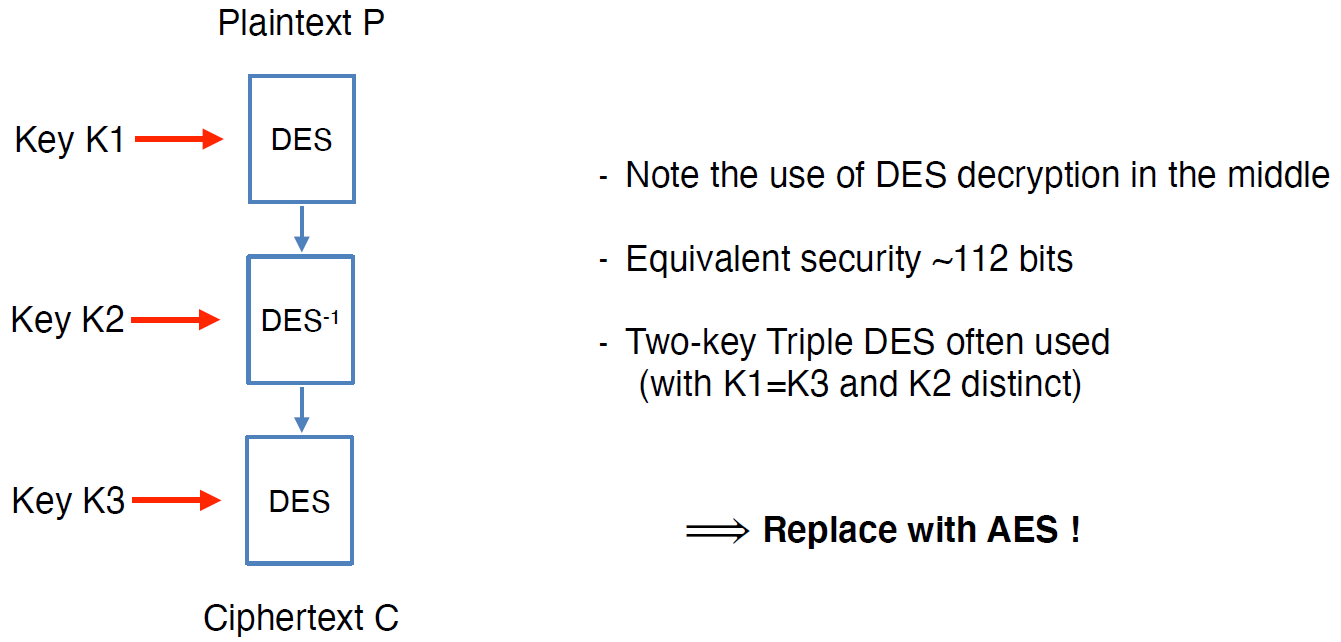
\includegraphics[width=140mm]{Graphics/Cryptanalysis/c3.png}
	\end{center}
	Because of the meet-in-the-middle attack on double DES, it turns out that to really get more security using multiple DES, we need to use triple DES. 
	In fact, triple DES still exists as a NIST standard, but will be disallowed after 2023. 
	Of course, we can still use this attack on triple DES to reduce its security to 112 bits (even if the overall key size is 168 bits). 
	Note that the attack now construct unbalanced lists, one of size $2^{56}$ (corresponding to the first key) and the other of size $2^{112}$ (corresponding to the last two keys). 
	Because of these unbalanced sizes, it is worth noting that there is a way to do the collision search that only requires a memory of the order of $2^{56}$ blocks. 
	Indeed, once the first list is constructed and sorted, we can build the second list one element at a time and use a dichotomy search to look for each element in the first list.\\
	Because the security can’t achieve 168 bits, the standard contains what is called two-keys triple DES, where the first and last keys are set to be identical. 
	Note that in the standard the middle invocation of DES decrypts with the second key rather than encrypt.
	It can be seen as a weakness. 
	For example, with two-key triple DES, if the first two keys are equal, the overall construction degenerates to simple DES. 
	In fact, this was done on purpose by NIST, to allow triple-DES equipment to perform simple DES by using this degenerate keys.\\
	You might still encounter triple DES in legacy applications, but it should be replaced by AES.

\section{Linear and Differential Cryptanalysis}
	\begin{itemize}
		\item The effort on studying DES (and other block ciphers like FEAL) led to:
		\begin{itemize}
			\item Differential Cryptanalysis (Biham/Shamir 1990)
			\item Linear Cryptanalysis (Matsui/Yamagishi 1992, Matsui 1993)\\
		\end{itemize}
		\item Both techniques consider probabilistic properties of the encryption:
		\begin{itemize}
			\item Found by examining building blocks
			\item Under the heuristic assumptions that events behave independently\\
		\end{itemize}
		\item These probabilistic techniques have been extended to other attacks
		\begin{itemize}
			\item Linear and differential remain essential for evaluating ciphers
		\end{itemize}
	\end{itemize}
	Two of the most fruitful methods that appeared by studying DES and some of the other block ciphers it inspired are the differential and the linear cryptanalysis techniques. 
	The first was invented by Biham and Shamir in 1990, the second two years later by Matsui and Yamagishi.\\
	These techniques share an important feature. 
	Indeed, both of them rely on observing probabilistic relations that are satisfied in the target block cipher more often than they would be in a random permutation. 
	Because of the large block sizes (and key sizes), such relations cannot be predicted by a brute force method. 
	Instead, they are first constructed on small building blocks of the cipher and then composed into a property of the block cipher (or of a reduced version of the cipher for some attacks).
	The composition techniques that are used are usually heuristic and rely on the assumption that successive rounds behave independently.\\
	They are many more recent attacks that share a lot of these features. 
	To name a few, we can cite the square attack, the boomerang attack or the impossible differential attack. 
	However, the linear and differential attacks remain essential to evaluate block ciphers and it is important to have some basic knowledge about them.

\section{Differential Cryptanalysis}
	\subsection{Fundamentals}
		\begin{center}
			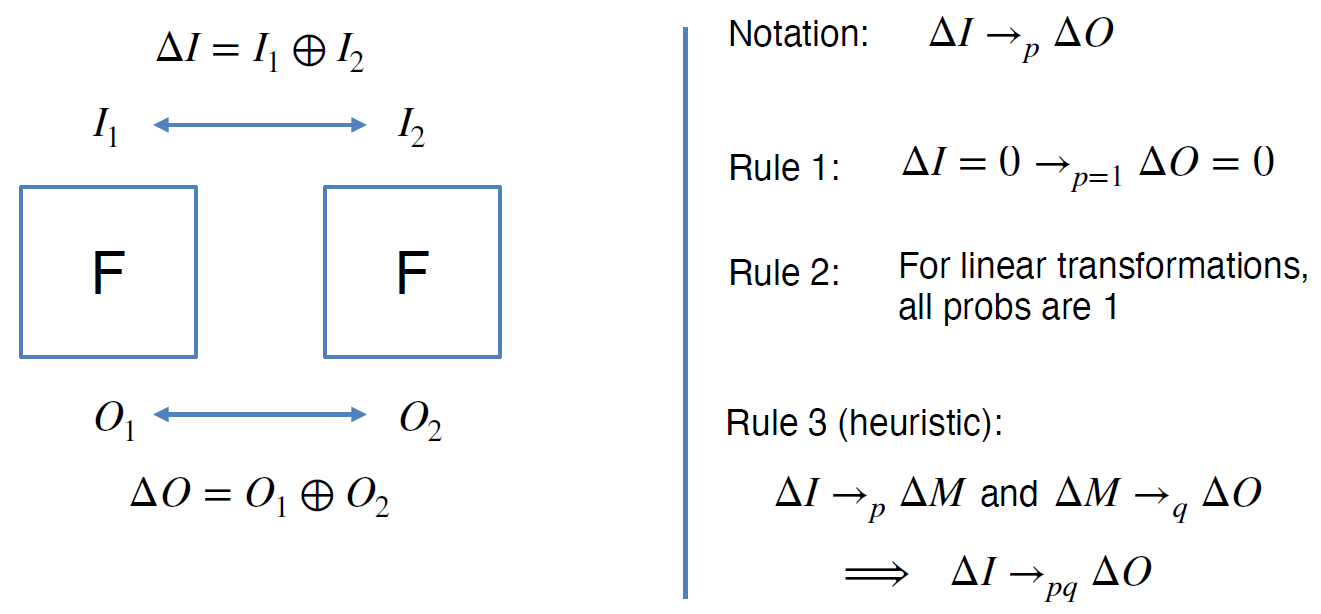
\includegraphics[width=140mm]{Graphics/Cryptanalysis/c4.png}
		\end{center}
		In the differential attack, we look at pairs of blocks, $I_1$ and $I_2$, that are encrypted into outputs $O_1$ and $O_2$. 
		The name differential comes from the fact that we study the relation between the difference of the inputs and the difference of the outputs. 
		Remember that, in our context, every block is formed of bit strings. 
		As a consequence, it is quite natural to study a bit-by-bit difference. 
		Moreover, when working with bits, operations modulo 2 are the most common choice. 
		Because of that, the difference of blocks is simply their Exclusive-OR.\\
		More precisely, for every possible input difference $\Delta I$, we count how many times it leads to an output difference, $\Delta O$. 
		After dividing by the number of possible pairs, we obtain the probability that $\Delta I$ leads to $\Delta O$. 
		We use the Notation at the top of the right column to indicate that $\Delta I$ leads to $\Delta O$ with probability $p$. 
		These probabilistic arrows are usually called differential characteristics.\\
		For example, for any block cipher (or any component of a block cipher), a zero difference in input always produce a zero difference in the output. 
		Similarly, for a linear transformation (on bits), the output difference is always the transformation by the linear map of the input difference.\\
		To be able to construct differential characteristics on a block cipher with many rounds, we need a way to compose probabilistic arrows. 
		For this, we use the third heuristic rule that says that we can combine two arrows where the output difference of the first is equal to the input difference of the second. 
		Moreover, the probability of the composition is the product of the individual probabilities, under the heuristic independence assumption.
	
	\subsection{Small example}
		Consider the ADD function with 2 input bits and 2 output bits:
		\begin{center}
			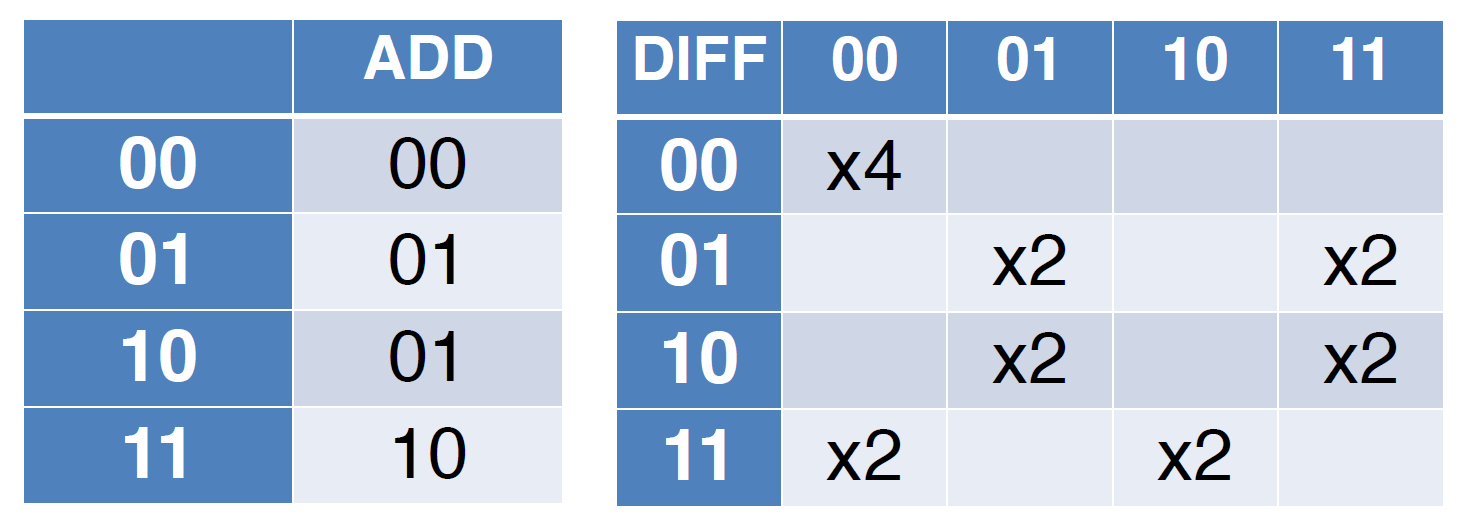
\includegraphics[width=140mm]{Graphics/Cryptanalysis/c5.png}
		\end{center}
		On this small example, we show a full table of differential counts for a function with two bits of input and two bits of output. 
		The chosen function is the addition of the two input bits, written in binary.\\
		The table on the right tells how many times each output difference appears for a given input difference and empty cells indicate that the corresponding output difference is not possible.
		
	\subsection{Principle of the attack}
		\begin{itemize}
		    \item Assume we have $\Delta I \to_p \Delta O$ for a block cipher (with $p >> 2^{-n}$)
		    \begin{itemize}
		        \item Encrypt many pairs with input difference
		        \item For the studied cipher $\Delta O$ is observed with probability close to $p$
		        \item For a random permutation $\Delta O$ is observed with probability close to $2^{-n}$\\
		    \end{itemize}
		    \item This yields a chosen plaintext distinguisher from a random permutation!\\
		    \item For key recovery, use the distinguisher on a restricted num of rounds
		    \item Together with exhaustive key search on (part of) the removed rounds
		\end{itemize}
		Once a differential characteristic is known for the full block cipher, we can build a distinguishing attack. 
		Namely, we are given access to an encryption device and want to determine whether it implements the target block cipher (with an unknown key) or a random permutation. 
		We simply encrypt many pairs with the prescribed input difference and observe how often the corresponding output occurs. 
		For the block cipher, the proportion is close to the probability $p$. 
		By contrast, for a random permutation, it is close to $2^{-n}$.\\
		The attack can also be used for key recovery. 
		For this, we start from a characteristic on a reduced number of rounds and query plenty of pairs with the prescribed input difference. 
		Then, we perform exhaustive search for the last round key, decrypt the output for one round and observe the difference. 
		For the correct guess, the prescribed output will occur more frequently. 
		There are subtleties to implement the attack when the key for the last round is too large for exhaustive search. 
		Indeed, in that case, the cryptanalysis needs to find a way to implement the attack using exhaustive search on a reduced part of the key.\\
		The details of how this can be done can vary depending on the exact specification of the block cipher we are attacking.


\section{Linear Cryptanalysis}
	\subsection{Fundamentals}
		\begin{center}
			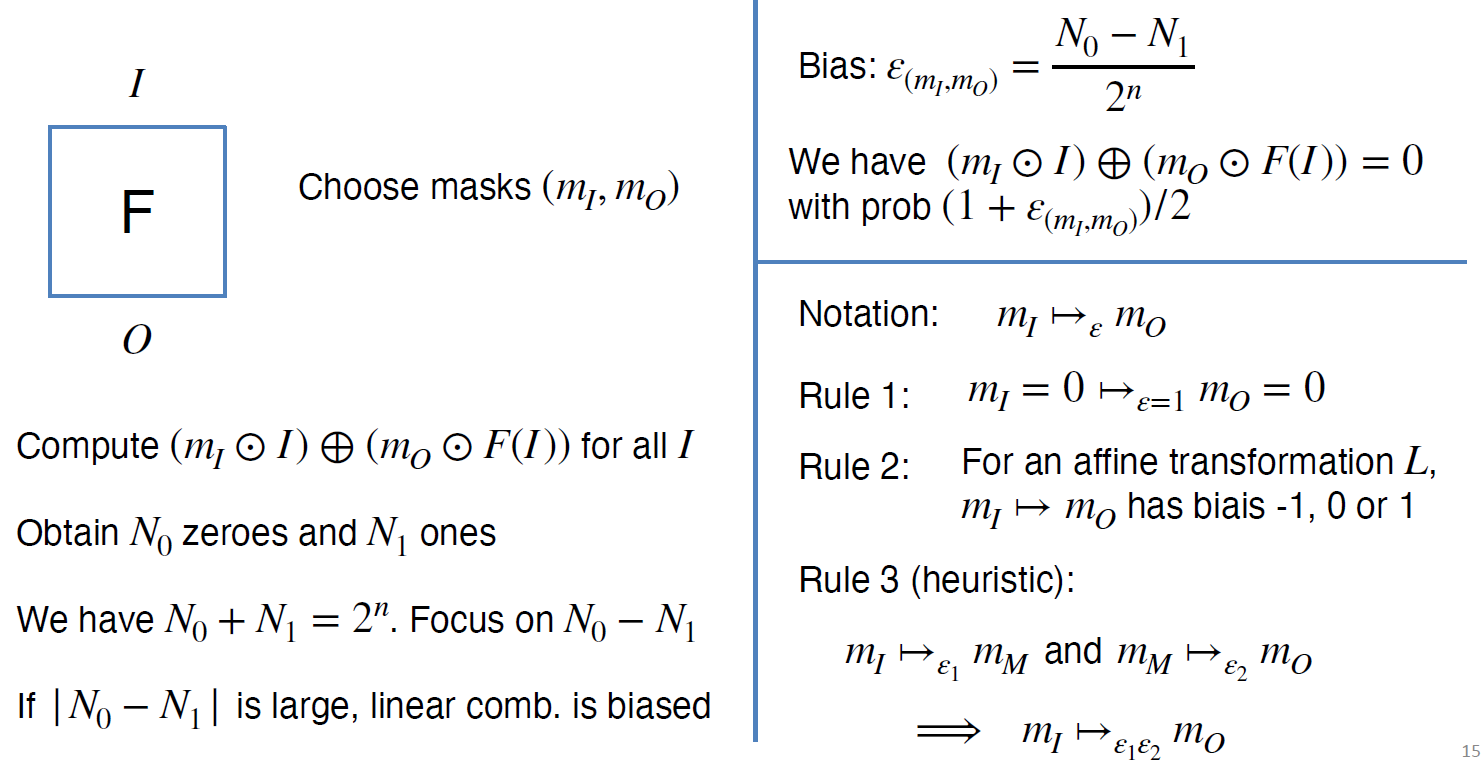
\includegraphics[width=140mm]{Graphics/Cryptanalysis/c6.png}
		\end{center}
		In linear cryptanalysis, we study the relation between inputs and outputs in a different way. 
		We choose two bit strings $m_I$ and $m_O$ (that we will call input and output mask) and, for input/output pairs $I-O$, 
		we study the distribution of the quantity ($m_I$ scalar $I$) XOR ($m_O$ scalar $O$). 
		In other words, we mask the input bits with the mask $m_I$ and the output bits with $m_O$, we count the number of '$1$' in the masked bit strings and compute the parity of this number, 
		namely we reduce the count modulo 2. 
		Over all inputs, let say that we observe a zero result $N_0$ times and a one result $N_1$ times. 
		Of course, $N_0 + N_1$ is equal to $2^n$, the total number of possible inputs. 
		Thus, the difference $N_0 - N_1$ encodes all the information we need about $N_0$ and $N_1$. 
		We now focus on this difference.\\
		When its absolute value is small, the result is balanced, that is zeroes and ones occur roughly as often as each other. 
		When it is large, there are much more zeroes or ones, depending on the sign of the difference.
		It is convenient to normalize the difference and consider the bias epsilon of $(m_I, m_O)$ which is defined as the difference divided by $2^n$. 
		Then, the probability to observe a zero is equal to (the bias +1) divided by two.
		Using a notation reminiscent of the one from differential cryptanalysis, we will write an arrow from $m_I$ to $m_O$ with the bias epsilon written as a subscript. 
		To avoid confusion, we use a different arrow in the notation.\\
		As before, there are some important rules that always hold. 
		First, for input and output masks equal to zero, we don’t observe any of the input bits or output bits. 
		As a consequence, the number of ones in this empty observation is always equal to zero and its parity is always zero. 
		Thus, the bias of this 0 to 0 arrow is equal to 1.\\
		For linear (and also affine) transformations, all arrows have bias equal to either 0, 1 or -1. 
		Showing this is a good exercise to become more familiar with the notion.\\
		The third rule is heuristic and consider a chain of two arrows, where the output mask of the first arrow is equal to the input mask of the second. 
		Then we have a composed arrow whose bias is the product of the biases of the initial ones.\\
		These rules can be used to construct linear characteristics for block ciphers built from many sub-components.
	
	\subsection{Small example}
		\begin{center}
			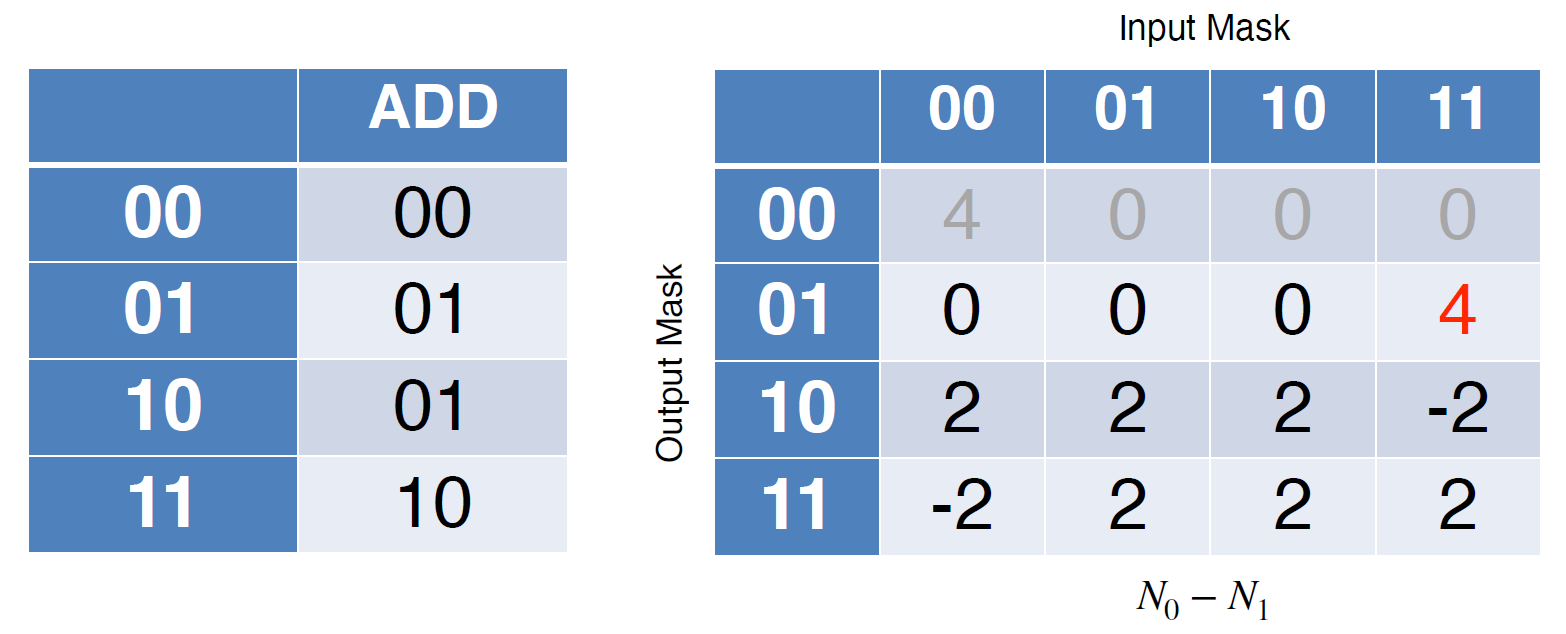
\includegraphics[width=140mm]{Graphics/Cryptanalysis/c7.png}
		\end{center}
		We now revisit our small example for linear cryptanalysis. 
		The first line is greyed out since the case of a zero output mask never provide any useful information because, in that case, we are not observing any of the output bits. 
		On the other hand, the first column where we do not observe the input bit can yield interesting information. 
		For exemple, the -2 at the bottom of the first column tells us that the XOR of the two output bits of an addition is more often equal to 1 than to 0. 
		The red 4 tells us that there is a linear relationship for input mask 11 and output mask 01.
		Indeed, the low order bit of a sum is equal to the XOR of the two input bits.

	\subsection{Principle of attack}
		\begin{itemize}
		    \item Assume we have $m_1 \mapsto_{\epsilon} m_0$ for a block cipher (with $\epsilon >> 2^{-n}$)
		    \begin{itemize}
		        \item Encrypt with inputs $I$ with output $O$, compute $(m_I \odot I) \oplus (m_O \odot O)$
		        \item For the studied cipher, large difference between num of zeroes and ones
		        \item For a random permutation, close to balance between zeroes and ones
		    \end{itemize}
		    \item This yields a known plaintext distinguisher from a random permutation!
		    \item For key recovery, we can take advantage of key mixed in using XORs
		\end{itemize}
		The principle of using linear cryptanalysis as a distinguisher is basically the same as the one we saw for differential cryptanalysis.\\
		However, for key recovery attacks, there is a very interesting twist. 
		This comes from the fact that in most block cipher, the key is incorporated by XOR it with intermediate values every now and then during the encryption process. 
		If we know a linear characteristic for a part of the cipher and want to XOR a key after this part, we can observe that this changes the value of the output scalar product 
		by a constant which is the parity of the number of ones in the corresponding key masked with the output mask. 
		This also composes well and as a consequence, the absolute value of bias of the global linear characteristic is unaffected by this specific way of introducing the key. 
		Only the sign will change (or not) depending on the value of one parity bit of the expanded key (coming from the key schedule).\\
		Of course, it is also possible to use the partial exhaustive search technique we described for differential cryptanalysis.

\section{Related Key attacks : Example of DES-X}
	\begin{center}
		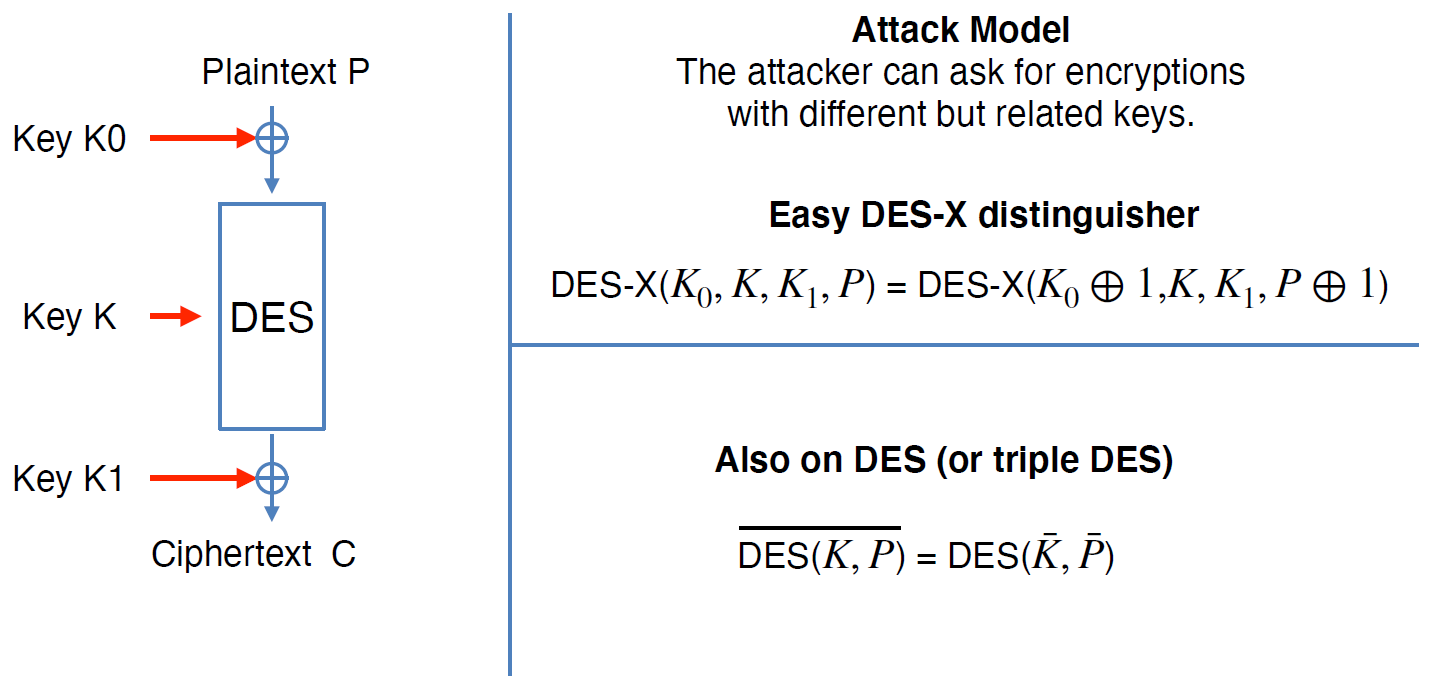
\includegraphics[width=140mm]{Graphics/Cryptanalysis/c8.png}
	\end{center}
	As a last example of block-cipher attacks, we now consider a new method called the related key attack. 
	It is a different attack model where the attacker can not only query the block cipher with its basic key but also with different but related keys obtained by XORing 
	the basic key with values which are arbitrarily chosen by the attacker. 
	It is also possible to replace XOR by another operation such as addition but care needs to be taken when defining the attack model.\\
	Related-key distinguishers arise naturally with some block ciphers. 
	A first example is the DES-X cipher proposed by Rivest to enlarge the key size of DES. 
	It consists in a sandwich structure where before and after DES encryption the plaintext and ciphertext blocks are XORed with two whitening keys K0 and K1.
	By itself it is an interesting technique that led to the Even-Mansour construction. 
	However, with DES-X, a related-key distinguisher can easily be built. 
	For example, it is clear that XORing any constant (let say 1) with both the plaintext block and the first whitening key while leaving everything else unchanged doesn’t change the ciphertext.\\
	Interestingly, there also is a simple related key distinguisher on DES itself. 
	Indeed, negating every bit of the plaintext and of the key at the same time creates a ciphertext which is the negation of the initial one.\\
	Related-key attacks may or may not be a problem in applications, it really depends on how the block-cipher is used. 
	However, block-cipher designers usually try to avoid them in order to prevent bad interactions in applications that could be vulnerable otherwise.

\section{Arbitrary related key attack model is too strong}
	\begin{center}
		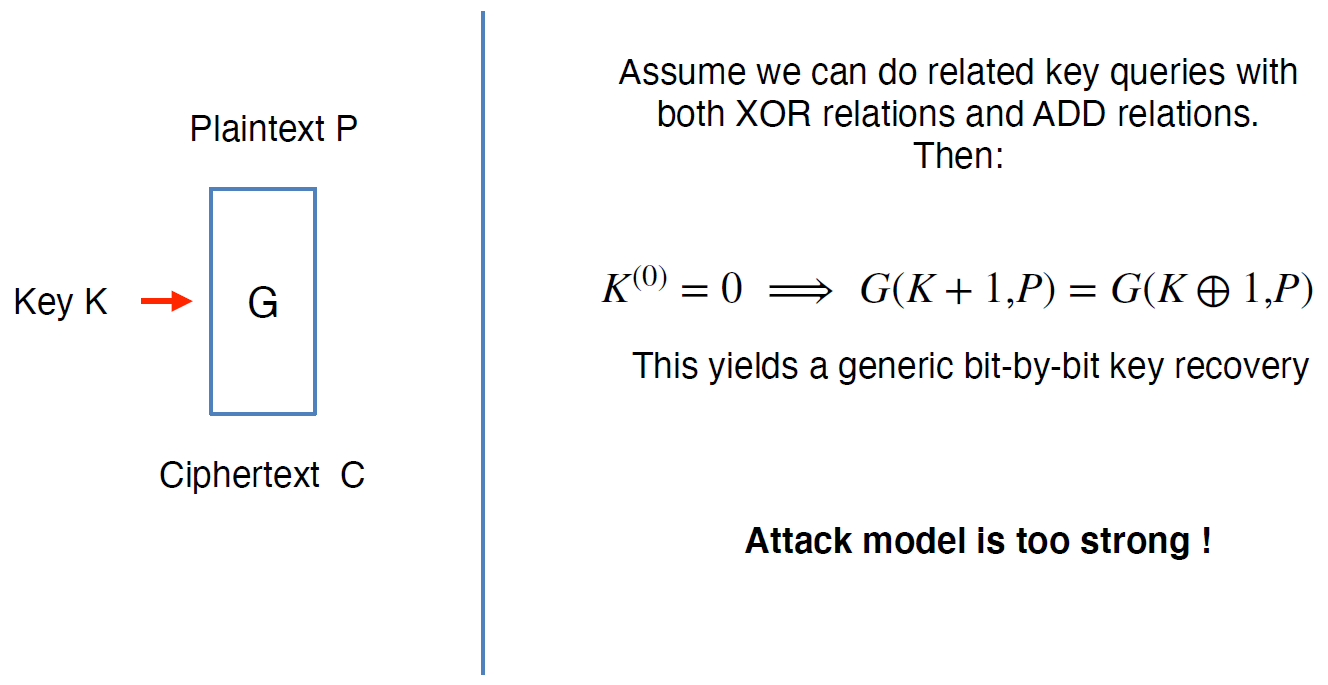
\includegraphics[width=140mm]{Graphics/Cryptanalysis/c9.png}
	\end{center}
	As mentioned in the previous slide, some care needs to be taken when considering related-key attacks. 
	Indeed, if the attacker is allowed to use arbitrary transforms of the initial key, there is an easy generic key recovery attack that becomes possible. 
	To show that assume that the adversary is allowed to either XOR the initial key with a constant of its choice or to ADD a chosen constant to the key (modulo $2^k$ where k is the key size).\\
	Remark that XORing the constant 1 to a key $K$ and adding 1 to the same key $K$ give the same result if and only if the lowest order bit of the key is a zero. 
	Moreover, testing if two keys are equal is easy to do by encrypting any plaintext block with both keys and comparing the resulting ciphertext blocks. 
	Thus, the adversary learns the first bit of the key. 
	By adding and XORing 2, 4, 8 and so on, he can also learn the remaining bits (with the exception of the top bit). 
	Of course, this exception is not a problem since once all the bits of the key except the last one are known, it suffices to test which of the two remaining possibilities is the correct key.\\
	As a consequence, when using related key attacks, one should always check that the model hasn’t been pushed in an extreme regime where this kind of generic attacks are possible.





























